% Exact LaTeX recreation of the supplied Phase-1.pdf
% Compile with pdfLaTeX. Place member pictures in the same folder if required.

\documentclass[11pt,a4paper]{article}

\usepackage[a4paper,left=2.0cm,right=2.0cm,top=1.55cm,bottom=1.55cm]{geometry}
\usepackage[T1]{fontenc}
\usepackage{lmodern}
\usepackage{graphicx}
\usepackage{xcolor}
\usepackage{array}
\usepackage{tabularx}
\usepackage{ragged2e}
\usepackage{enumitem}
\usepackage{fancyhdr}
\usepackage{tikz}
\usepackage{setspace}

% -------------------------------------------------
% COLOURS
% -------------------------------------------------
\definecolor{TitleBlue}{RGB}{61,103,154}

% -------------------------------------------------
% GENERAL SETTINGS
% -------------------------------------------------
\setlength{\parindent}{0pt}
\setlength{\parskip}{0pt}
\renewcommand{\arraystretch}{1.0}

% The supplied document uses a clean sans-serif heading style
% and italic serif-style explanatory text.
\newcommand{\blueheading}[1]{%
    {\sffamily\color{TitleBlue}\fontsize{15}{18}\selectfont #1}%
}

\newcommand{\bluebigheading}[1]{%
    {\sffamily\bfseries\color{TitleBlue}\fontsize{16}{19}\selectfont #1}%
}

\newcommand{\instruction}[1]{%
    {\itshape\fontsize{10.5}{12.5}\selectfont #1}%
}

\newcommand{\answerbox}[2][3.0cm]{%
    \vspace{2pt}
    \noindent
    \fbox{%
        \begin{minipage}[t][#1][t]{\dimexpr\textwidth-2\fboxsep-2\fboxrule\relax}
            \vspace{1mm}
            \itshape #2
        \end{minipage}
    }
}

% -------------------------------------------------
% HEADER / FOOTER
% -------------------------------------------------
\pagestyle{fancy}
\fancyhf{}
\renewcommand{\headrulewidth}{0pt}
\renewcommand{\footrulewidth}{0pt}

\fancyhead[L]{%
    \sffamily\bfseries\itshape\fontsize{10.5}{12}\selectfont
    COURSE NAME AND ID
}
\fancyhead[R]{%
    \sffamily\bfseries\fontsize{10.5}{12}\selectfont
    PROJECT PROPOSAL
}
\fancyfoot[R]{%
    \itshape\fontsize{10}{12}\selectfont
    Page \thepage
}
\setlength{\headheight}{14pt}
\setlength{\headsep}{23pt}
\setlength{\footskip}{24pt}

% -------------------------------------------------
% PAGE 1
% -------------------------------------------------
\begin{document}

\vspace*{4mm}

\bluebigheading{PROJECT AND TEAM INFORMATION}

\vspace{13mm}

\blueheading{Project Title}

\answerbox[1.0cm]{Smart Garbage Collection & Route Optimization}

\vspace{13mm}

\blueheading{Student / Team Information}

\vspace{2mm}

\noindent
\begin{tabularx}{\textwidth}{
    |>{\RaggedRight\arraybackslash}p{0.62\textwidth}
    |>{\RaggedRight\arraybackslash}p{0.38\textwidth}|
}
\hline

% =================================================
% TEAM NAME
% =================================================
\begin{minipage}[t]{\linewidth}
\vspace{3mm}
\textit{Team Name:}\\[-1mm]
\textit{Team \#}
\vspace{3mm}
\end{minipage}
&
\begin{minipage}[t]{\linewidth}
\vspace{3mm}
\textit{Avengers}
\vspace{3mm}
\end{minipage}
\\
\hline

% =================================================
% TEAM MEMBER 1
% =================================================
\begin{minipage}[t][3.55cm][t]{\linewidth}
\vspace{3mm}
\textbf{Team member 1 (Team Lead)}\\[1mm]
\textit{(Last Name, name: student ID: email, picture):}
\end{minipage}
&
\begin{minipage}[t][3.55cm][t]{\linewidth}
\vspace{3mm}
\textit{Singh, Manthan --}\\
\textit{2510350070}\\
\textit{smanthan236@gmail.com}

\vspace{2mm}
\includegraphics[width=2.5cm,height=1.25cm,keepaspectratio]{PHOTO-2026-09-02-22-00-26.jpg}
\end{minipage}
\\
\hline

% =================================================
% TEAM MEMBER 2
% =================================================
\begin{minipage}[t][3.55cm][t]{\linewidth}
\vspace{3mm}
\textbf{Team member 2}\\[1mm]
\textit{(Last Name, name: student ID: email, picture):}
\end{minipage}
&
\begin{minipage}[t][3.55cm][t]{\linewidth}
\vspace{3mm}
\textit{Rana, Aryan --}\\
\textit{2510350073}\\
\textit{aryanrana811@gmail.com}

\vspace{2mm}
\includegraphics[width=2.5cm,height=1.25cm,keepaspectratio]{PHOTO-2026-09-02-22-07-34.jpg}
\end{minipage}
\\
\hline

% =================================================
% TEAM MEMBER 3
% =================================================
\begin{minipage}[t][3.55cm][t]{\linewidth}
\vspace{3mm}
\textbf{Team member 3}\\[1mm]
\textit{(Last Name, name: student ID: email, picture):}
\end{minipage}
&
\begin{minipage}[t][3.55cm][t]{\linewidth}
\vspace{3mm}
\textit{Singh, Shaurya Pratap --}\\
\textit{2510011689}\\
\textit{shauryapratapsingh@gmail.com}

\vspace{2mm}
\includegraphics[width=2.5cm,height=1.25cm,keepaspectratio]{show-3.jpg}
\end{minipage}
\\
\hline

% =================================================
% TEAM MEMBER 4
% =================================================
\begin{minipage}[t][3.55cm][t]{\linewidth}
\vspace{3mm}
\textbf{Team member 4}\\[1mm]
\textit{(Last Name, name: student ID: email, picture):}
\end{minipage}
&
\begin{minipage}[t][3.55cm][t]{\linewidth}
\vspace{3mm}
\textit{Hritambra -- 2510380105}\\
\textit{riturawat442@gmail.com}

\vspace{2mm}
\includegraphics[width=2.5cm,height=1.25cm,keepaspectratio]{PHOTO-2026-09-02-21-57-45.jpg}
\end{minipage}
\\
\hline

\end{tabularx}

\newpage

% -------------------------------------------------
% PAGE 2
% -------------------------------------------------

\bluebigheading{PROPOSAL DESCRIPTION (10 pts)}

\vspace{12mm}

\blueheading{Motivation (1 pt)}

\vspace{1mm}

\answerbox[3.3cm]{
Municipal solid waste collection today relies on fixed schedules and routes, with trucks visiting
every bin regardless of how full it actually is — a problem visible at every scale. Globally, MSW
generation is projected to rise from 2.1 to 3.8 billion tonnes by 2050 (a 56% increase), with
management costs nearly doubling to USD 640 billion, while 29–33% of waste already goes
uncollected or mismanaged (UNEP, World Bank). In India, CPCB (2024) data shows ~170,000
tonnes generated daily, but only 54% is actually treated, with cities projected to hit 435 million
tonnes annually by 2050. Locally, Dehradun generates ~350 metric tonnes/day, yet the Municipal
Corporation can only transport about 80% regularly — leaving a daily backlog dumped or burned,
causing public-health and environmental hazards.
}
\vspace{1mm}

\blueheading{State of the Art / Current solution (1 pt)}

\vspace{1mm}

\answerbox[5.15cm]{
\vspace{.3mm}
Currently the municipal is still stuck to manual solution to this problem that is still using the fixed routes on
daily or alternative basis and overdumping of waste in some trucks while leaving some trucks as partially
empty. Current solution that are introduced uses ultrasonic IOT sensors, some example comes from
Antariksh Waste Ventures (IIT-Madras incubated, "Airbin") and SenRa have built ultrasonic/load-cell
sensor bins using LoRa/NBIoT connectivity, results are strong: a 2024 study across 10 sites in Lahore,
Pakistan measured a 32% improvement in route efficiency, 29% lower fuel consumption, and 18%
maintenance savings versus fixed routes. Globally, Bigbelly, Sensoneo, and Ecube Labs offer full
commercial platforms (solar compactors + sensors + routing software), with Ecube Labs explicitly entering
the Indian market. But there is a catch to this solution! existing solutions (Bigbelly, Sensoneo, Ecube Labs) are
costly, hardware-dependent, and impractical for small-scale use, many pilots lack automated route
optimization, relying on manual decisions. We are targeting to fill this gap by our project
}

\vspace{13mm}

\blueheading{Project Goals and Milestones (2 pts)}

\vspace{1mm}

\answerbox[9.50cm]{
Our goal is to build a simulation system that models a set of garbage bins with live or simulated
fill‑ level data. The simulation system will automatically spot which garbage bins are urgent and
will compute the efficient collection route for a truck that can carry only so much. This approach
should show, with numbers such as distance travelled bins overflowed and truck capacity usage
that it beats a fixed‑ route baseline.

\begin{itemize}[leftmargin=*,nosep]
    \item Milestone 1: Create Bin and Truck classes using design then generate or simulate fill‑ level data for
the garbage bins.
    \item Milestone 2: Build threshold‑ based filtering and a priority queue that ranks garbage bins by how
full they're
    \item Milestone 3: Use a graph‑ based route‑ optimization algorithm such as nearest‑ neighbour with the
option to extend to Dijkstra to order the urgent garbage bins for the truck starting from its current
spot.
    \item Milestone 4: Add truck capacity limits so that the truck returns to the depot when full then
continues collecting.
    \item Milestone 5: Create console or graphical output that displays the status of each garbage bin, the
chosen route and a clear before‑ and‑ after comparison, with the fixed‑ route baseline showing
distance saved and bins that were kept from overflowing.
\item Milestone 6: Perform testing, write documentation. Produce the final report and demonstration
\end{itemize}
}
\vspace{22mm}

\vspace{12mm}

\blueheading{Project Approach (3 pts)}

\vspace{1mm}

\answerbox[7.3cm]{
The system will be implemented in C++ using Object-Oriented Programming and core Data Structures, in
line with the course's DSA-in-C and OOP-in-C++ components. Two main classes will be modeled: Bin (id,
coordinates, fill level) and Truck (current position, capacity, assigned route), with a supporting Graph
structure representing bins and roads as nodes and weighted edges. Bin fill-level data will be simulated
(randomized or read from a CSV file) to mimic real IoT sensor input, keeping the design open to future
integration with real sensors. A threshold value (e.g. 70%) will separate 'urgent' bins from normal ones;
urgent bins will be pushed into a priority queue (max-heap by fill percentage) so the most critical bins are
always considered first — an O(log n) insertion/extraction operation that scales well as the number of bins
grows. A greedy nearest-neighbor algorithm will then compute the visiting order: starting from the truck's
position, always move to the closest unvisited urgent bin (Euclidean distance, or shortest-path distance via
Dijkstra's algorithm on the road graph, O((V+E) log V)), until capacity is reached or all urgent bins are
served. The console output will display the fixed-route vs. dynamic-route comparison, with concrete
numbers (total distance, bins collected, bins at overflow risk) to demonstrate efficiency gains.
}
\vspace{2mm}

% -------------------------------------------------
% PAGE 3
% -------------------------------------------------
% -------------------------------------------------
% SYSTEM ARCHITECTURE
% -------------------------------------------------

\blueheading{System Architecture (High Level Diagram)(2 pts)}

\vspace{1mm}


\vspace{2mm}

\noindent
\fbox{%
\begin{minipage}[t]{\dimexpr\textwidth-2\fboxsep-2\fboxrule\relax}

\vspace{3mm}

\begin{center}
\textbf{\sffamily
Smart Garbage Collection \& Route Optimization - System Architecture}
\end{center}

\vspace{2mm}

\begin{center}
\resizebox{0.96\textwidth}{!}{%
\begin{tikzpicture}[
    box/.style={
        draw,
        rounded corners=3pt,
        minimum width=4.0cm,
        minimum height=1.45cm,
        align=center,
        font=\sffamily\bfseries\small,
        text=white
    },
    arrow/.style={
        ->,
        >=stealth,
        thick
    },
    label/.style={
        font=\sffamily\tiny
    }
]

% -------------------------------------------------
% TOP ROW
% -------------------------------------------------

\node[box, fill=TitleBlue] (input) at (0,3.2)
{Data Input Layer\\
(Random sim / CSV /\\
Manual entry)};

\node[box, fill=green!55!black] (bin) at (5.0,3.2)
{Bin Objects\\
(Bin class:\\
id, x, y, fill \%)};

\node[box, fill=green!55!black] (priority) at (10.0,3.2)
{Priority Module\\
(priority\_queue,\\
threshold filter)};

\node[box, fill=orange!80!black] (route) at (15.0,3.2)
{Route Optimizer\\
(greedy nearest-\\
neighbor search)};

% -------------------------------------------------
% BOTTOM ROW
% -------------------------------------------------

\node[box, fill=TitleBlue] (store) at (0,0)
{Bin Data Store\\
(CSV / DB log)};

\node[box, fill=violet!75!black] (truck) at (10.0,0)
{Truck Object\\
(Truck class: position,\\
capacity, route)};

\node[box, fill=violet!75!black] (output) at (15.0,0)
{Output Display\\
(console route +\\
stats log)};

% -------------------------------------------------
% ARROWS - TOP
% -------------------------------------------------

\draw[arrow] (input.east) -- node[above,label] {fill \%} (bin.west);

\draw[arrow] (bin.east) -- node[above,label] {urgent bins} (priority.west);

\draw[arrow] (priority.east) -- node[above,label] {priority list} (route.west);

% -------------------------------------------------
% ARROWS - BOTTOM / FEEDBACK
% -------------------------------------------------

\draw[arrow] (input.south) -- node[right,label] {log} (store.north);

\draw[arrow] (store.north east) -- node[above left,label] {history} (bin.south west);

\draw[arrow] (truck.north) -- node[right,label] {current state} (priority.south);

\draw[arrow] (route.south) -- node[right,label] {optimized route} (output.north);

\draw[arrow] (output.west) -- node[above,label] {route + stats} (truck.east);

\end{tikzpicture}
}
\end{center}

\vspace{3mm}

\begin{center}
\textit{\fontsize{8}{10}\selectfont
Note: bin data is software-simulated (no physical sensor hardware)
-- Bin and Truck are C++ OOP classes.}
\end{center}

\vspace{2mm}

\noindent
\textit{
Bin fill levels are generated in software through a Data Input Layer
(random simulation, CSV file, or manual entry) rather than physical
sensors, and are stored as attributes of Bin objects (id, coordinates,
fill \%) defined by the Bin class. The Priority Module filters and ranks
these Bin objects above the urgency threshold using a priority queue.
The Route Optimizer applies a greedy nearest-neighbor search, using the
Truck object's current position and capacity (defined by the Truck class),
to produce an ordered pickup route. The result is written to an Output
Display (console route and statistics log), and the Truck object's updated
position and load feed back into the Priority Module to keep the system
state current -- all handled entirely through OOP classes, with no physical
sensor hardware involved.
}

\vspace{6mm}

\end{minipage}
}

\vspace{40mm}

\blueheading{Project Outcome / Deliverables (1 pts)}

\vspace{1mm}

\answerbox[4.7cm]{\item  A working C++ console application demonstrating dynamic bin prioritization and route
generation.
\item  Bin, Truck, and Graph classes with clean OOP structure (encapsulation, modularity, STL
usage).
\item  A quantified comparison report showing distance/fuel/time saved versus a fixed-route
baseline, using sample data (e.g. Bin A 20%, Bin B 96%, Bin C 72%, Bin D 15%, Bin E 91%)
and benchmarked against published pilot results (~30% route efficiency gain, ~29% fuel
reduction, per cited studies).
\item  Source code, README, and final project report with complexity analysis of algorithms
used (priority queue O(log n), Dijkstra O((V+E) log V), greedy routing).
\item  A short demo/presentation showing the system responding to changing bin fill levels in
real time.}

\vspace{12mm}

\blueheading{Assumptions}

\vspace{7mm}

\answerbox[3.65cm]{We assume bin fill-level data is either simulated with randomized values or manually entered, in
place of real IoT sensors (due to hardware unavailability) — this is consistent with how most
academic and early-stage smart-waste prototypes are validated before hardware deployment.
We assume a single truck with a fixed known capacity for the base version, and a 2D coordinate
map with Euclidean distance (or a small weighted graph) as an approximation of real road
distances. Traffic conditions, multiple simultaneous trucks, and real-time GPS integration are
considered out of scope for the base version but are addressed as planned extensions below.}

\vspace{12mm}

\blueheading{References}

\vspace{1mm}

\answerbox[7.65cm]{● Central Pollution Control Board (CPCB), Govt. of India, 2024, via CEEW — "How can
Indian Cities Boost Sustainable Solid Waste Management?"
(https://www.ceew.in/publications/how-can-indian-cities-boost-sustainable-solid-waste-
management-practices) — India's daily MSW generation, collection, and treatment
figures; 2050 projection.
\item  FleetRabbit — Smart Waste Management with IoT Sensors, 2026
(https://fleetrabbit.com/blogs/post/smart-waste-management-iot-sensors) — fleet-level
trip/fuel/overflow reduction figures.
\item  GeeksforGeeks — Priority Queue, Dijkstra's Algorithm, and Greedy Algorithms
(https://www.geeksforgeeks.org/)
\item  Bigbelly Smart Waste Solutions — https://bigbelly.com/ ; Sensoneo Smart Waste
Management — https://sensoneo.com/
\item  Herbert Schildt: “The Complete Reference C++”, 4th Edition, Tata McGraw Hill, 2003
\item  R. Kruse etal, “Data Structures and Program Design in C” Pearson Education}

\end{document}
